\chapter{Analýza požadavků}

\textit{Tato kapitola popisuje požadavky, jež byly kladeny na vývoj systému.}

Jak již bylo zmíněno v úvodu, cílem práce je vyrobit webovou aplikaci, jež komunikuje se serverem a je schopna číst konfigurace na základě kterých pak vizualizuje grafová data. Konfigurace a serverová část byla napsána mým vedoucím a tedy sloužila jako specifikace systémových požadavků na klientskou část. V následující podkapitole nejprve popíšu strukturu konfigurace.

\section{Konfigurace}

\subsection{Rozšíření požadavků}
Původní návrh konfigurací byl mírně jednodušší a považoval konfigurace pouze jako odkazy na seznam pohledů. Klientská aplikace tedy musela mít seznam konfigurací s jejich názvy počátečními vrcholy a dalšími parametry. Na základě debaty s mým vedoucím jsem se rozhodl konfigurace rozšířit o tyto parametry (název, počáteční vrcholy) a přidat meta konfigurace, jež slouží jako složky pro konfigurace. Níže je tedy popsán již nový návrh konfigurací.

\bigskip

V následujících sekcích jsou použity tyto RDF namespacy:
\begin{table}[h] \centering
\begin{tabular}{lp{10cm}}
\toprule
\multicolumn{1}{c}{Prefix} & \multicolumn{1}{c}{IRI}                                      \\
\midrule
browser                    & \texttt{\url{https://linked.opendata.cz/ontology/knowledge-graph-browser/}} \\
dct                        & \texttt{\url{http://purl.org/dc/terms/}}
\end{tabular}
\end{table}

\subsection{Meta konfigurace} \label{pozadavky-metakonfigurace}
Meta konfigurace je skupina pro další konfigurace a meta konfigurace. Díky tomuto uživatel může procházet desíkty různých konfigurací uspořádaných do složek obdobně jak v souborovém systému na počítači. Meta konfigurace má tyto vlastnosti:

\begin{itemize}
    \item \texttt{dct:title} Název metakonfigurace \textit{(je možné zadat ve více jazycích)}
    \item \texttt{dct:description} Detailnější popis, co daná metakonfigurace obsahuje \textit{(je možné zadat ve více jazycích)}
    \item \texttt{browser:image} Odkaz na URL soubor s obrázkem reprezentujícím metakonfiguraci. Obrázek je pak zobrazen v aplikaci při procházení konfigurací.
    \item \texttt{browser:hasMetaConficuration} Meta konfigurace, které spadají pod tuto meta konfiguraci. \textit{(je očekáváno více objektů)}
    \item \texttt{browser:hasConfiguration} Konfigurace, které spadají pod tuto metakonfiguraci. \textit{(je očekáváno více objektů; popsáno dále)}
\end{itemize}

Meta konfigurací může být například \uv{Wikidata} nebo \uv{Otevřená data ČR}.

\subsection{Konfigurace} \label{pozadavky-konfigurace}
Konfigurace popisuje, jak by měla aplikace procházet datasety. Dvě konfigurace již byly zmíněny v úvodní kapitole. Aktuálně může mít konfigurace tyto vlastnosti:

\begin{itemize}
    \item \texttt{dct:title} Název konfigurace \textit{(je možné zadat ve více jazycích)}
    \item \texttt{dct:description} Detailnější popis, čeho je možné s konfigurací dosáhnout \textit{(je možné zadat ve více jazycích)}
    \item \texttt{browser:hasVisualStyleSheet} Určuje, jak mají uzly v aplikaci vypadat. \textit{(popsáno dále)}
    \item \texttt{browser:startingNode} Doporučený uzel nebo uzly, kde začít s procházením grafu. \textit{(je očekáváno více objektů)}
    \item \texttt{browser:resourceUriPattern} Regulární výraz popisující, jak by mělo vypadat IRI uzlu. Používá se v aplikaci jako nápověda uživateli, zda zadal správné IRI ještě než se pošle požadavek.
    \item \texttt{browser:hasViewSet} View sety. \textit{(popsáno dále)}
    \item \texttt{browser:autocomplete} JSON soubor se seznamem RDF uzlů podle kterých probíhá hledání. \textit{(je očekáváno více objektů; popsáno dále)}
\end{itemize}

\subsection{ViewSet} \label{pozadavky-view-sets}
View set reprezentuje skupinu pohledů. Pravý smysl pohledů pochopí čtenář dále v textu. View set má následující vlastnosti:
\begin{itemize}
    \item \texttt{dct:title} Název view setu \textit{(je možné zadat ve více jazycích)}
    \item \texttt{browser:hasView} Pohledy které patří pod tento view set. \textit{(je očekáváno více objektů; popsáno dále)}
    \item \texttt{browser:hasDefaultView} Výchozí pohled ze seznamu výše.
    \item \texttt{browser:hasCondition} SPARQL ASK dotaz jež určí, zda tato množina pohledů je aplikovatelná na konkrétní uzel.
    \item \texttt{browser:hasDataset} Dataset vůči kterému probíhá ASK dotaz. \textit{(popsáno dále)}
\end{itemize}

\subsection{View}
Konkrétní pohled na uzel jež byl vysvětlen v úvodu. View má následující vlastnosti:

\begin{itemize}
    \item \texttt{dct:title} Název pohledu \textit{(je možné zadat ve více jazycích)}
    \item \texttt{dct:description} Popis pohledu \textit{(je možné zadat ve více jazycích)}
    \item \texttt{browser:hasExpansion} Odkaz na expanzi - určuje jaké uzly lze získat z daného uzlu \textit{(popsáno dále)}
    \item \texttt{browser:hasPreview} Odkaz na preview - určuje jaká data se mají získat pro ostylování konkrétního uzlu \textit{(popsáno dále)}
    \item \texttt{browser:hasDetail} Odkaz na detail - určuje která data se zobrazí v detailu konkrétního uzlu \textit{(popsáno dále)}
\end{itemize}

\subsection{Expansion} \label{pozadavky-expansion}
Expansion popisuje jak lze daný uzel expandovat, tedy jedná se o operaci kdy se stahují nové uzly jež jsou nějak příbuzné expandovanému uzlu. Expanze vrací graf, tedy expandované uzly nemusí být přímými sousedy expandovaného. Jako expanzi si můžeme představit například \uv{Zobraz všechny knihy co napsala daná osoba}. Expanze formálně partří k pohledu (view).
\begin{itemize}
    \item \texttt{dct:title} Název expanze \textit{(je možné zadat ve více jazycích, aktuálně se nepoužívá)}
    \item \texttt{browser:hasDataset} Popisuje dataset vůči kterému se dotazuje na data. \textit{(popsáno dále)}
    \item \texttt{browser:query} Popisuje SPARQL SELECT dotaz který bude spuštěn na endpointu datasetu.
\end{itemize}

\subsection{Preview} \label{pozadavky-preview}
Preview popisuje která data v rámci daného pohledu (view) popisují daný uzel. Popisem se myslí taková data, kretá mají na svědomí stylování uzlu. V aplikaci je možné mít uzly různých barev a tvarů, to právě popisuje preview. Obdobně jako expanze, preview patří ke konkrétnímu pohledu.

Preview má stejné vlastnosti jako expanze. \texttt{browser:query} v tomto případě popisuje SPARQL dotaz, který vrátí graf obsahující daný uzel a jeho literály a z těchto literálů bude sestaven preview.

Konkrétně pro preview je predikát \texttt{browser:class} považován na třídy uzlu a ty jsou nastaveny jako třídy v knihovně Cytoscape\footnote{\url{https://js.cytoscape.org/}}, která je využíváná v klientské části na krelsení grafů.

\subsection{Detail} \label{pozadavky-detail}
Detail je poslední z trojice a poskytuje dodatečné informace k uzlu. Může se jednat o literály které nemá smysl v dané konfiguraci vykreslit do grafu jako uzly, proto budou zobrazeny v bočním panelu aplikace.

Detail má stejné vlastnosti včetně \texttt{browser:query} jako preview.

\subsection{Dataset} \label{pozadavky-dataset}
Dataset popisuje SPARQL endpoint vůči kterému probíhá dotazování na data.

\begin{itemize}
    \item \texttt{dct:title} Název datasetu \textit{(aktuálně se nepoužívá)}
    \item \texttt{void:sparqlEndpoint} URL adresa SPARQL endpointu na kterou se posílají SPARQL dotazy
    \item \texttt{browser:accept} Popisuje HTTP Accept type v jakém formátu by měl endpoint svá data poskytnout. \todo{nemělo by to čistě záležet na serveru?}
\end{itemize}

\subsection{Visual style sheet} \label{pozadavky-visual-style-sheet}
Popisuje jakž styl mají mít uzly v dané konfiguraci. Popis je založen na datech pocházejících právě z \textbf{preview}. Forma zápisu stylů aktuálně odpovídá stylům jaké používá knihovna Cytoscape.

Visual style sheet má pouze jednu vlastnosti

\begin{itemize}
    \item \texttt{browser:hasVisualStyle} Jedno pravidlo jak se má provést stylování, odkazuje na \textbf{Visual style}.
\end{itemize}

\subsubsection{Visual style}
Visual style má pak:

\begin{itemize}
    \item \texttt{browser:hasSelector} Selector pro Cytoscape knihovnu, jež vybírá \\ na které uzly nebo hrany daný styl bude aplikován.
    \item \texttt{browser:*} Jednotlivá pravidla jak má být daný uzel nebo hrana ostylována. Používají se přesně ty názvy, které používá knihovna Cytoscape, kupříkladu \texttt{browser:border-width} nebo \texttt{browser:background-color}.
\end{itemize}

\begin{figure}
    \centering
    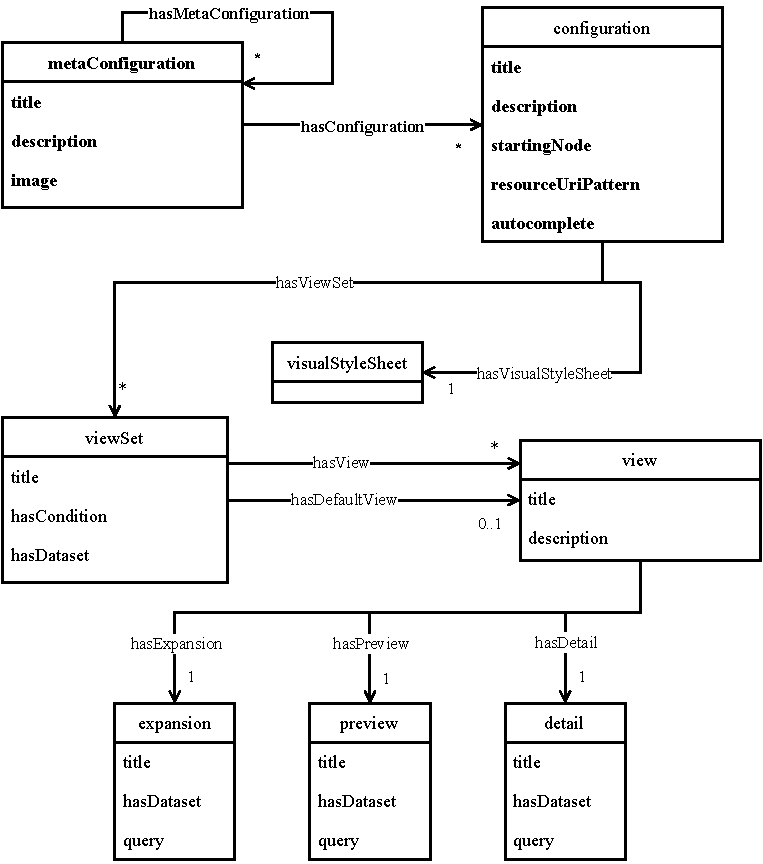
\includegraphics{media/configuration-class-diagram.pdf}
    \caption{Class diagram konfigurací. Tučně jsou zvýrazněné části jež nebyli součásti původní specifikace.}
    \label{fig:configuration-class-diagram}
\end{figure}

\newpage





\section{Server}
Funkcionálním požadavkem bylo, aby aplikace komunikovala se serverem, který provádí dotazy a vrací data pro aplikaci. Server bude detailněji popsán v příští kapitole.

Server zprostředkovává následující požadavky:
\begin{itemize}
    \item \texttt{/meta-configuration} - Vrátí informace o meta konfiguraci

    \item \texttt{/configuration} - Vrátí informace o konfiguraci

    \item \texttt{/stylesheet} - Vrátí visual style sheet

    \item \texttt{/view-sets} - K vrcholu a konfiguraci vrátí seznam view setů

    \item \texttt{/preview} - K vrcholu a pohledu vrátí preview

    \item \texttt{/detail} - K vrcholu a pohledu vrátí detail

    \item \texttt{/expand} - K vrcholu a pohledu vrátí expandované uzly
\end{itemize}

\newpage





\section{Uživatelské a systémové požadavky}

Níže je sepsán seznam původních požadavků na klientskou aplikaci.

\subsection{Konfigurace a stylesheet}
Uživatel musí být schopen vybrat IRI konfigurace a visual style sheetu a lze je kdykoli změnit. IRI konfigurace může být vybráno jen jedno.

\paragraph{Analýza} Konfigurace popisuje, jak je graf zobrazen a které pohledy jsou na uzly aplikovatelné. Není tedy možné mít dvě konfigurace v jednom grafu a změnou konfigurace tedy dojde ke smazání původního grafu.

\subsection{Vložení vrcholů}
Uživatel může ručně zadat IRI vrcholu který se následně zobrazí v grafu.

\paragraph{Analýza} Pro úspěšné zobrazení vrcholu musí aplikace znát preview vrcholu. Preview lze ale získat pouze z konkrétního pohledu a je tedy nutné nejprve stáhnout view sety daného vrcholu, z nich následně vybrat defaultní a zvolit výchozí pohled. Pak je možné zavolat metodu \texttt{preview} na serveru a získat data o uzlu.

IRI uzlu budeme považovat za chybné, pokud server vrátí prázdnou množinu view sets. V takovém případě totiž nejde aplikovat žádné pohledy na uzel a tedy zřejmě nepatří do dané konfigurace.

Vrchol může být již v grafu přítomen, pak bude viditelně zvýrazněn. Pokud je uzel skrytý, bude odkryt. Pokud jsou zapnuté filtry a uzel je skrytý filtrem, uzel se v grafu nezobrazí. Pokud se uzel podaří načíst, nebo již existuje, bude vybrán a zobrazí se jeho detail v pravém panelu.

\subsection{Detail vrcholu}
Pokud uživatel klikne na vrchol, zobrazí se panel s podrobnými informacemi o uzlu. Bude zobrazen detail uzlu voláním metody \texttt{detail} na serveru a budou zobrazeny veškeré pohledy vrcholu, možnost je přepínat a provádět expanze podle daného pohledu.

Detail bude zobrazen jako dvousloupcová tabulka klíč-hodnota.

Panel bude zobrazovat také další možné akce k vrcholu.

\paragraph{Analýza} Vrchol nemusí mít načtené view sets, preview ani detail, je tedy nutné po zobrazení panelu tyto informace stáhnout a během stahování zobrazit informaci, že se data stahují.

Může se stát, že \texttt{view-sets} vrátí prázdný výsledek. V takovém případě vrchol v grafu necháme i přes to, že podle původního požadavku bychom jej smazali.

Mezi akcemi bude lokalizace vrcholu, smazání, znovunačtení všech dat, zafixování pozice.

\subsection{Skrývání uzlů}
Uživatel může skrývat uzly v panelu s detailem. Skrytý uzel se v grafu skryje společně se všemi hranami a bude možné zobrazit seznam skytých uzlů ze kterého bude možné skryté uzly opět zviditelnit.

\paragraph{Analýza} Bude přidáno tlačítko k detailu pro skrytí/zobrazení uzlu. Současně pro vetší přehlednost bude do detailu přidána hláška informující uživatele, že je uzel skrytý.

Skryté uzly nebude možno lokalizovat ale stále bude možné s nimi dále pracovat. Podle prvního požadavku se uzel opět zobrazí, pokud ho uživatel bude chtít explicitně vložit.

V panelu se skrytými uzly bude možnost uzly přímo zobrazit, nebo si zobrazit jejich detail. Detail skrytého uzlu funguje stejně jako pro viditelné uzly.

\subsection{Expanze}
Po dvojkliku na uzel se uzel expanduje podle aktuálního pohledu. Uzel je také možné expandovat v panelu s detailem kliknutím na tlačtko expanze u příslušného pohledu. Expanzí se zavolá metoda \texttt{expand} na serveru a v grafu se zobrazí nové vrcholy.

\paragraph{Analýza} Pokud přidávaný vrchol v grafu již je a je skrytý, pak skrytým zůstane. Na rozdíl od přidávání jednoho vrcholu totiž explicitně neříkáme, že chceme daný vrchol přidat. Protože je možné vrcholy mazat, povolíme uživateli provádět expanzi znova, i když byla provedena.

\paragraph{Poznámka} Aktuálně se expanze ukládají k vrcholům a je tedy možné zjistit, které vrcholy vznikly ze které expanze bez nutnosti znovu expanzi volat. Bohužel tato funkcionalita ještě není implementována a je řešena v poslední kapitole.

\subsection{Filtrování vrcholů}
Uživatel může přidat filtr, jež skryje nevyhovující vrcholy. Takovéto skryté vrcholy se pak chovají stejně jako uživatelem skryté vrcholy. Požadované filtry jsou
\begin{itemize}
    \item Zobraz jen ty vrcholy, jež mají stupeň v daném intervalu nebo rozmezí.
    \item Zobraz vrcholy jen s konkrétním typem nebo třídou.
\end{itemize}

\paragraph{Analýza} Aplikace by měla podporovat snadné přidání filtrů do budoucna a podporu pro pluginy, které dodávají vlastní možnosti filtrování. Aby bylo možné vyjádřit libovolné filtry, každý filtr by měl mít přístup k celému grafu a všem vrcholům.

Uzel může být skrytý jak filtrem, tak i uživatelem. Pro přehlednost by měl být uživatel informován, že nemůže ručně zobrazit vrchol který je skrytý filtrem. Tyto vrcholy budou stále zobrazeny v seznamu skrytých vrcholů pro možnost přístupu k nim.

Každý filtr určí, zda je vrchol podle tohoto filtru viditelný. Vrchol pak bude viditelný pokud všechny filtry určí, že viditelný je. Jedná se tedy o konjunkci.

Typy a třídy vrcholů nejsou známy předem a API serveru neumožňuje získat celou množinu typů a tříd. Je tedy nutné přizpůsobit filtry tak, aby si dokázaly poradit s novými uzly. Proto filtry na typ a třídu budou mít dva módy, v jednom módu explicitně skrývají zvolené vlastnosti a ve druhém explicitně zobrazují vrcholy s danými vlastnostmi. Toto chování pak ovlivní přidání nových, neznámých, vrcholů. V prvním případě nový vrchol bude zobrazen (pokud jeho typ, resp. třídy ještě nejsou známy) a ve druhém případě bude ihned skryt.

\subsection{Vícejazyčné uživatelské rozhraní}
Uživatel může přepínat mezi více jazyky uživatelského rozhraní. Aktuálně bude podporována pouze angličtina a čeština.

\paragraph{Analýza} Kromě uživatelského rozhraní by měl být vícejazyčný i graf. Aktuální API serveru toto ještě neumožňuje a problém je předmětem poslední kapitoly. Multijazyčnost zatím podporují metody \texttt{meta-configuration} a \texttt{configuration} na serveru. Protože obecně můžou existovat překlady do spousty světových jazyků, je vhodné stahovat pouze požadovaný jazyk a při jeho změně stáhnout nový jazyk. Podrobněji je toto rozebráno v kapitole s implementací. \todo{ref}

Pro velké grafy může být překlad problémem, protože změna jazyku může vyvolat spoustu požadavků na datové zdroje. Pro překlad grafu by tedy bylo nejlepší stáhnout překlad až když si uživatel zobrazí detail, nebo explicitně neoznačí vrcholy na překlad. Taktéž je vhodné oddělit výběr jazyka pro obsluhu aplikace a výběr konfigurací od překladu jednotlivých vrcholů. Příkladem může být procházení měst v Japonsku anglicky mluvícím uživatelem, kdy je žádoucí, aby názvy měst byly v originále.

\subsection{Stažení grafu do souboru}
Uživatel má možnost stáhnout aktuální graf do souboru a později ho ze souboru načíst zpět.

\paragraph{Analýza} Protože je aplikace ve vývoji, je třeba dbát na zpětnou kompatibilitu. Při každé nové verzi je tedy třeba ověřit, že soubor pochází ze staré verze a použít staré metody pro jeho zpracování a převedení do nového systému. Výsledný soubor může být zkomprimován pro menší velikost a nabízí se i možnost stáhnout jen základní informace tak, aby zbytek mohl být při načtení stažen ze serveru. Toto je opět řešeno v poslední kapitole.

Pokud uživatel bude chtít zavřít aplikaci, bude dotázán, zda chce aktuální graf uložit do souboru. Uložený graf již nebude blokovat stránku o uzavření dokud uživatel nesmaže, nebo nepřidá nové uzly. Stažení detailu, nebo změna pohledu nebude považována za změnu hodnou k uložení.

Pokud uživatel zvolí načtení nového souboru, starý graf bude zahozen a uživatel tedy bude požádán o uložení.

Kromě otevření souboru ze systému bude možnost soubor našíst i z webu.

\begin{figure}
    \centering
    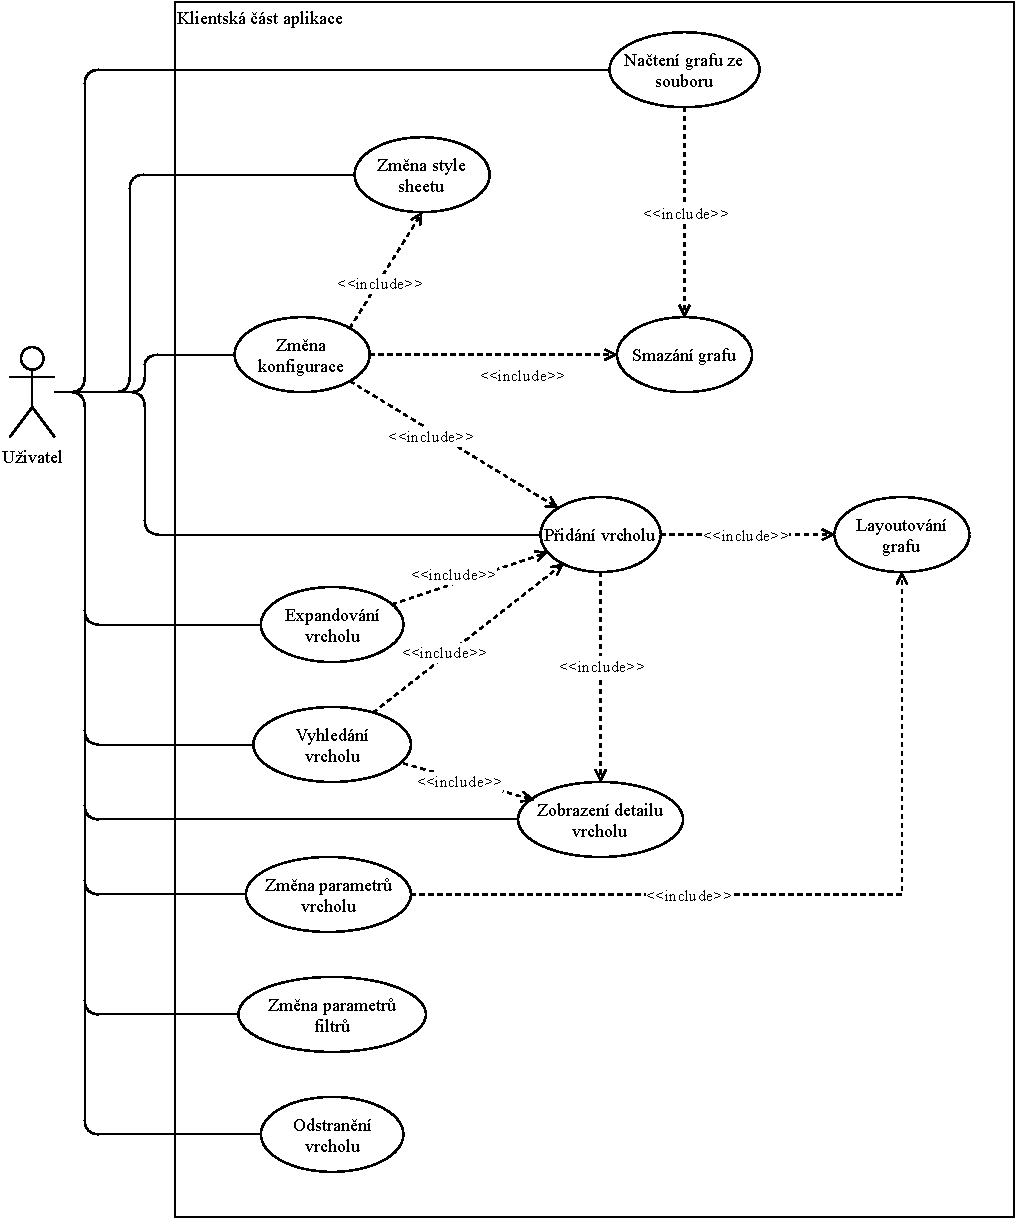
\includegraphics[width=\textwidth]{media/use-case.pdf}
    \caption{Use case diagram vytváření grafu a základní práce s grafem.}
    \label{fig:use-case}
\end{figure}

\newpage

\subsection{Odstranění vrcholu}
Uživatel může z grafu vrchol odstranit.

\paragraph{Analýza} Odstraněním vrcholu se musí odstranit i všechny hrany patřící vrcholu.

Odstranit vrchol bude možné pomocí tlačítka v panelu s detailem, popřípadě skupinu vrcholů bude možné odstranit obdobným způsobem.

\subsection{Vyhledávání vrcholů s pomocí autocomplete}
Pokud to konfigurace umožňuje, bude možné přidávat nové uzly do grafu s pomocí autocomplete.

\paragraph{Analýza} Data pro vyhledávání se budou stahovat až když uživatel bude chtít poprvé vyhledávat.

\subsection{Podpora layoutů}
Aplikace bude umožňovat několik způsobů layoutování grafu, které si bude moci uživatel volit.

\begin{itemize}
    \item Pokud to layout umoňuje, bude možné ukotvit vrchol. To lze provést přesunutím vrcholu nebo pravým kliknutím myši. U ukotvených vrcholů bude zobrazena ikonka. Takovéto vrcholy pak nebudou layoutem ovlivněny.
    \item Layout reaguje na různé události, jako vytvoření skupiny, expanze vrcholu, přidání nového vrcholu do grafu, přesunutí vrcholu a na základě těchto událostí provádí layoutování grafu.
    \item Pokud to layout umožňuje, bude v pravém dolním rohu obrazovky tlačítko které spustí layoutování explicitně.
    \item Layout má vlastní nastavení.
\end{itemize}

\subsection{Seskupování vrcholů}
Vrcholy bude možné seskupovat do skupin které budou ve vizuálním grafu reprezentovány jedním uzlem. Pokud expanze vrátí větší množství nových vrcholů, vzniknou jako skupina. Skupinu bude možné rozbít dvojklikem.

\begin{itemize}
    \item Z grafového hlediska skupina vzikne kontrakcí hran mezi vrcholy skupiny. To znamená, že pokud vedla hrana mezi vrcholem mimo skupinu a vrcholem ve skupině, povede tato hrana mezi vrcholem mimo skupinu a skupinou. Všechny násobné hrany stejného typu budou odstraněny. Obdobně toto platí i mezi dvěma skupinama. Pokud je ve skupině vrchol skrytý (ať uživatelem, nebo filtrem), jeho hrany se nepodílejí na utváření skupiny. Pokud jsou všechny vrcholy skupiny skryty, je skrytá i skupina.
    \item Skupina se na grafu chová jako obyčejné vrhcholy, je ji možné skrýt, přesouvat, ukotvit atp.
    \item Označením několika vrcholů se nabídne možnost vytvořit skupinu. Tato skupina pak vzikne na místě, kde byly původní vrcholy.
    \item Rozbít skupinu je možné dvojklikem, nebo tlačítkem z detailu skupiny. Vrchol skupiny bude odstraněn a vziknou místo něj původní vrcholy, které budou layoutovány.
\end{itemize}
